%%  pdflatex bmle.tex 
%%  bibtex bmle.aux 
%%  pdflatex bmle.tex 
%%  pdflatex bmle.tex
%% pdflatex bmle.tex && bibtex bmle.aux && pdflatex bmle.tex && pdflatex bmle.tex


%\documentclass[a4paper,12pt]{}
\documentclass[final, paper=letter,5p,times,twocolumn]{elsarticle}
%\documentclass[preprint,review,8pt,times]{elsarticle}


%% or use the graphicx package for more complicated commands
%\usepackage{changebar}
\usepackage{graphicx}
\usepackage{caption}
\usepackage{subcaption}
\usepackage{multirow}
%% or use the epsfig package if you prefer to use the old commands
%% \usepackage{epsfig}

%% The amssymb package provides various useful mathematical symbols
\usepackage{tikz}
\usepackage{amsmath,amsfonts,amsthm,multicol,bm} % Math packages
\usepackage{mathtools, cuted}
%\usepackage{dsfont} % mathds{1}
%\usepackage{widetext} % 
\usepackage{listings}
\usepackage{amssymb}
\usepackage{hyperref}
%
%\usepackage[]{algorithm2e}
%% Macro
\newcommand{\ToDo}[1]{ToDo: \textbf{\textit{#1}}}
\newcommand{\CA}{computational anatomy}
%
\newtheorem{theorem}{Theorem} % reset theorem numbering for each section
\newdefinition{definition}{Definition}%

\theoremstyle{definition}
%\newtheorem{defn}[thm]{Definition} % definition numbers are dependent on theorem numbers
\newtheorem{example}[theorem]{Example} % same for example numbers

%\newtheorem*{example}{Example}
%\newtheorem{theorem}{Theorem}%
\newtheorem{corollary}{Corollary}[theorem]
\newtheorem{lemma}[theorem]{Lemma}
%\newproposition{proposition}{Proposition}%
%\newlemma{lemma}{Lemma}%
%\AtEndEnvironment{theorem}{\null\hfill\qedsymbol}%

\begin{document}
%%%%%%%%%%%%%%%%%%%%%%%%%%%%%%%%%%%%%%%%%%%%%%%%%%%%%%%%%%%%%%%%%%%%%%%%%%
%%%%%%%%%%%%%%%%%%%%%%%%%%%%%%%%%%%%%%%%%%%%%%%%%%%%%%%%%%%%%%%%%%%%%%%%%%
%%%%%%%%%%%%%%%%%%%%%%%%%%%%%%%%%%%%%%%%%%%%%%%%%%%%%%%%%%%%%%%%%%%%%%%%%%
%%%%%%%%%%%%%%%%%%%%%%%%%%%%%%%%%%%%%%%%%%%%%%%%%%%%%%%%%%%%%%%%%%%%%%%%%%
\begin{frontmatter}

\title{Bayesian Mixted Linear Effect}

\author[label1]{Yann Cobigo\corref{cor1}}
\address[label1]{University of California, San Francisco | ucsf.edu}
%\address[label2]{Address Two\fnref{label4}}

%\cortext[cor1]{I am corresponding author}
%\fntext[label3]{I also want to inform about\ldots}
%\fntext[label4]{Small city}

\ead{yann.cobigo@ucsf.edu}
\ead[url]{https://github.com/YannCobigo}

%% \author[label5]{Author Two}
%% \address[label5]{Some University}
%% \ead{author.two@mail.com}
%% 
%% \author[label1,label5]{Author Three}
%% \ead{author.three@mail.com}

\begin{abstract}
In this report we will present the model based rate of atrophy. The model will be contrained to a longitudinal data acquisition over several years and different age subject having different variant of frontotemporal lobar dementia (FTLD). The model will be fitted with a Bayesian Mixted Linear algorithm.
\end{abstract}

\begin{keyword}
%% keywords here, in the form: keyword \sep keyword
Bayesian Mixted Linear Effect \sep parametric empirical Bayes \sep Model based atrophy
%% MSC codes here, in the form: \MSC code \sep code
%% or \MSC[2008] code \sep code (2000 is the default)
\end{keyword}

\end{frontmatter}

%%%%%%%%%%%%%%%%%%%%%%%%%%%%%%%%%%%%%%%%%%%%%%%%%%%%%%%%%%%%%%%%%%%%%%%%%%
%%%%%%%%%%%%%%%%%%%%%%%%%%%%%%%%%%%%%%%%%%%%%%%%%%%%%%%%%%%%%%%%%%%%%%%%%%
%%%%%%%%%%%%%%%%%%%%%%%%%%%%%%%%%%%%%%%%%%%%%%%%%%%%%%%%%%%%%%%%%%%%%%%%%%
%%%%%%%%%%%%%%%%%%%%%%%%%%%%%%%%%%%%%%%%%%%%%%%%%%%%%%%%%%%%%%%%%%%%%%%%%%

\section{Introduction}

\paragraph{MRI blabla}{MRI best for {\it in-vivo} study, cost, long run longitudinal study.}

\paragraph{Mixted Linear Effect blabla}{A lot of study has been done in a cross-sectional fashion, some study appears with longitudinal inference on the slop of the atrophy rate. Possibility to assess group difference and each individual within the same framework (random-effect).}

\paragraph{Bayesian treatment blabla}{The conditional mean can be caracterize for each level of the hierarchical model. At the lowest level, the bayesian model characterizes the model parameters witht the same accuracy as a Maximum-Likelyhood algorithm (ML).}

%%%%%%%%%%%%%%%%%%%%%%%%%%%%%%%%%%%%%%%%%%%%%%%%%%%%%%%%%%%%%%%%%%%%%%%%%%
%%%%%%%%%%%%%%%%%%%%%%%%%%%%%%%%%%%%%%%%%%%%%%%%%%%%%%%%%%%%%%%%%%%%%%%%%%
\section{Model Based Atrophy Rate}

We considere the rate of atrophy as being a polynomial function $r$. Each unit of time a tissue $a$ decreases from $V_{t=i}$ to $V_{t=j}$:

\begin{equation*}
  \left .
  \begin{array}{rcl}
    V_{0} & \rightarrow & V_{1} = V_{0} - r \times V_{0} \\
    V_{1} & \rightarrow & V_{2} = V_{1} - r \times V_{1} = (1-r)^{2}V_{0} \\
    V_{2} & \rightarrow & V_{3} = V_{2} - r \times V_{2} = (1-r)^{3}V_{0} \\
  \end{array}
  \right .
\end{equation*}

After $t$ unit of time, the volume is $V(t) = V_{0}\exp(t \times \ln(1-r))$.\\


At a maturity stage of life we considere the Total Intracranial volume (TIV) as being constant and the gray matter fully devloped \ToDo{ref which age?}. After this maturity age gray and white matter decreases in volume, then cerebrospinal fluid (CSF) volume increases: $V_{TIV} = V_{gm} + V_{wm} + V_{csf} = n_{gm}V_{TIV} + n_{wm}V_{TIV} + n_{csf}V_{TIV}$ where $V_{TIV}$ represents the TIV, $V_{gm}$ and $n_{gm}$ the gray matter volume and proportion of the TIV, $V_{wm}$ and $n_{wm}$ the white matter volume and proportion of the TIV, and $V_{csf}$ and $n_{csf}$ the CSF volume and proportion of the TIV. 

\paragraph{$V_{0}$ problematics}{The first probelmatic brought with a model like $V(t) = V_{0}(1 - r(t))^{t}$ is we don't know what represents $V_{0}$ or when $t=t_{0}$ has to be considered. We can considere a cannonical age when the skull is supposed to have reached the threasholding age, then the gray matter is $V(t=t_{0}) = V_{0} = n_{gm}TIV$. Another possibility is to create a temaplate targetting a mean age $t = <age>$ (the best would be close to the oldest age of subjects not seek, 40 years old for instance). At the voxel level we can state $V_{0,i} = \alpha_{i}V_{T,i}$, where $V_{0,i}$ is the normalized, modulated subject's gray matter intensity in the voxel $i$, $V_{T,i}$ represents the template intensity at the voxel $i$, $\alpha_{i}$ represents the proportionality coefficient between the subject and the template at the voxel level. Then the model can be written:

  \begin{equation}
    \left .
    \begin{array}{rcl}
      V_{i}(t) & = & \alpha_{i}V_{T,i} (1 - r_{i}(t))^{t}
    \end{array}
    \right .
    \label{template_model_based}
  \end{equation}

  The logarithm of the former expression, using a very weak rate of atrophy

  \begin{equation}
    \left .
    \begin{array}{rcl}
      \ln\frac{V_{i}(t)}{V_{T,i}} & = & \ln(\alpha_{i}) + t \times \ln(1 - r_{i}(t)) \\
      & \sim & \ln(\alpha_{i}) - t \times \left(r_{i}(t) + \frac{1}{2} r_{i}^{2}(t) + \cdots \right)
    \end{array}
    \right .
    \label{log_template_model_based}
  \end{equation}

  Mostlikely, with the instrument precision the rate will be seen as a constant. We develop the model to be a first degree lenear model in each voxel $r_{i}(t) = a + bt$ the case where the model is constant is easely derived from the affine model.

    \begin{equation}
    \left .
    \begin{array}{rcl}
      \arg & = & \ln(\alpha_{i}) + t \times \left \lbrack -a - bt - \frac{1}{2} \left(  a + bt \right)^{2} \right \rbrack \\
      & = & \ln(\alpha_{i}) + t \times \left \lbrack -a - bt - \frac{1}{2}  a^{2} - abt - \frac{1}{2}(bt)^{2} \right \rbrack \\
    \end{array}
    \right .
    \label{affine_rate_atrophy_model}
  \end{equation}

  
}

%%%%%%%%%%%%%%%%%%%%%%%%%%%%%%%%%%%%%%%%%%%%%%%%%%%%%%%%%%%%%%%%%%%%%%%%%%
%%%%%%%%%%%%%%%%%%%%%%%%%%%%%%%%%%%%%%%%%%%%%%%%%%%%%%%%%%%%%%%%%%%%%%%%%%
\section{Hierarchical models}

\ToDo{talk. parametric empirical Bayes (PEB)} \\
\ToDo{talk. } \\
\ToDo{talk. } \\

The statistical will be based on a time-dependant PEB hierarchical model over $(n)$ levels:

\begin{equation}
  \left .
  \begin{array}{rcl}
    Y & = & X^{(1)} \theta^{(1)} + \epsilon^{(1)} \\
    \theta^{(1)}& = & X^{(2)} \theta^{(2)} + \epsilon^{(2)} \\
    \vdots && \\
    \theta^{(n-1)}& = & X^{(n)} \theta^{(n)} + \epsilon^{(n)} \\
  \end{array}
  \right .
  \label{hierarchical_model}
\end{equation}

The matrix $Y$ represents the measure at every voxel for different time-points. the matrix $X^{(i)}$ represent the design matrix for the level $i$ embeding the explanatory variables and higher level constriants. The matrix $\theta_{i}$ are the level parameters and $\epsilon^{(i)}$ is the error at the level $i$. The error is supposed to be a Gaussian noise $\epsilon^{(i)} \sim \mathcal{N}(0,C_{\epsilon}^{i})$ with null mean and covariance $C_{\epsilon}^{i}$.\\
The model (\ref{hierarchical_model}) can be written recursively in the following matter:

\begin{equation}
  \left .
  \begin{array}{rcl}
    Y & = & \epsilon^{(1)} +  X^{(1)} \epsilon^{(2)} + \cdots + X^{(1)} \cdots X^{(n-1)} \epsilon^{(n)}   \\
    & + & X^{(1)} \cdots X^{(n)} \theta^{(n)}\\
    & = & X\theta + \epsilon^{(1)} 
  \end{array}
  \right .
  \label{hierarchical_model_recursive}
\end{equation}

In the Baysian framework, $X = [X^{(1)}, \cdots, X^{(1)} \cdots X^{(n)}]$ and $\theta = [\epsilon^{(2)}, \cdots, \epsilon^{(n)}, \theta^{(n)}]^{T}$. The form (\ref{hierarchical_model_recursive}) has the following covariance matrix:

\begin{equation}
  \left .
  \begin{array}{rcl}
    E\{YY^{T}\} & = & \underset{error}{\underbrace{C_{\epsilon}^{(1)}}} +  \underset{random~effects~level~2}{\underbrace{X^{(1)} C_{\epsilon}^{(2)} X^{(1)T}}} + \cdots \\
    & + & \underset{random~effects~level~i}{\underbrace{X^{(1)} \cdots X^{(i-1)} C_{\epsilon}^{(i)} X^{(i-1)T} \cdots X^{(1)T}}}  \\
    & + & \cdots + \underset{fixed~effects}{\underbrace{X^{(1)} \cdots X^{(n)} C_{\theta}^{(n)}X^{(n)T} \cdots X^{(1)T}}} \\
    & = & C_{\epsilon}^{(1)} + XC_{\theta}X^{T} \\
  \end{array}
  \right .
  \label{hierarchical_cov_recursive}
\end{equation}

where

\begin{equation}
  Cov\{\theta\} = C_{\theta} = \left (
  \begin{array}{cccc}
   C_{\epsilon}^{(2)} & \cdots & 0 & 0\\
   \vdots & \ddots & \vdots & \vdots \\
   0 & \cdots & C_{\epsilon}^{(n)} & 0 \\
   0 & \cdots & 0 & C_{\theta}^{(n)}\\
  \end{array}
  \right )
  \label{C_theta}
\end{equation}

and

\begin{equation}
  E\{\theta\} = \eta_{\theta} = \left (
  \begin{array}{c}
   0 \\
   \vdots  \\
   0  \\
   \eta_{\theta}^{(n)}\\
  \end{array}
  \right )
  \label{eta_theta}
\end{equation}


In the PEB framework, we set an infinit covariance for the highest level: $C_{\theta}^{(n)} = \infty$ (unknown).

%%%%%%%%%%%%%%%%%%%%%%%%%%%%%%%%%%%%%%%%%%%%%%%%%%%%%%%%%%%%%%%%%%%%%%%%%%
\subsection{Maximum \`a posteriori}

The baysian inference is based on the conditional probability distribution of the parameters, $p(\theta^{(i)}|Y)$, at a level $(i)$ given the data. We assume our data are distributed arround the model with a gaussian distribution and our parameters, at each level, are also \`a priori distributed in a gaussian manner. Since the likelyhood and the parameters \`a priori are gaussian distributed, we assume the posterior distribution will also be gaussian distributed (\ToDo{site Bishop}). The Bayse rule can be written

\begin{equation}
  p(\theta | Y) =   p(Y | \theta) p(\theta) / p(Y) 
\end{equation}

In the remainer of the manuscript, the marginal probability $p(Y)$ will be ignored. The PEB offers, at a level $(i)$, inferences of the gaussian first and second moments: $\eta_{\theta|Y}^{(i)}$ and $C_{\theta|Y}^{(i)}$, representing the maximum \`a prosteriori (MAP). The level $(i)$ is thought as prior constraints on the expectation and the covariance


\begin{equation}
  \left .
  \begin{array}{rcl}
    E\{\theta^{(i-1)}\}   & = & \eta_{\theta}^{(i-1)} = X^{(i)}\theta^{(i)} \\
    Cov\{\theta^{(i-1)}\} & = & C_{\theta}^{(i-1)} = C_{\epsilon}^{(i)}\\
  \end{array}
  \right .
  \label{Prior_constraint}
\end{equation}

The likelyhood and the priors can be written with the gaussian distribution using the precision matrix ($\Lambda^{(i)} = C^{(i)-1}$):


\begin{equation*}
  \left .
  \begin{array}{rcl}
    p(Y|\theta) & \propto & \exp\lbrace -\frac{1}{2} (X\theta - Y)^{T} \Lambda_{\epsilon}^{(1)} (X\theta - Y) \rbrace \\
    p(\theta)   & \propto & \exp\lbrace -\frac{1}{2} (\theta - \eta_{\theta})^{T} \Lambda_{\theta} (\theta - \eta_{\theta}) \rbrace \\
  \end{array}
  \right .
\end{equation*}

The distribution \`a posteriori is

\begin{equation*}
  \left .
  \begin{array}{rcl}
    p(\theta|Y) & \propto & \exp\lbrace -\frac{1}{2} (\theta - \eta_{\theta|Y})^{T} \Lambda_{\theta|Y} (\theta - \eta_{\theta|Y}) \rbrace \\
  \end{array}
  \right .
\end{equation*}

Where

\begin{equation}
  \left .
  \begin{array}{rcl}
    \Lambda_{\theta|Y} & = & X^{T}\Lambda_{\epsilon}^{(1)}X + \Lambda_{\theta}\\
    & = &
    \left (
    \begin{array}{cccc}
      \Lambda_{\epsilon|Y}^{(2)} & \cdots & & \\
      \vdots & \ddots && \\
      && \Lambda_{\epsilon|Y}^{(n)} & \\
      &&& \Lambda_{\theta|Y}^{(n)}  \\
  \end{array} 
    \right ) \\
    \eta_{\theta|Y}  & = & C_{\theta|Y} \left( X^{T}\Lambda_{\epsilon}^{(1)}Y + \Lambda_{\theta}\eta_{\theta} \right)\\
    & = &
    \left (
    \begin{array}{c}
      \eta_{\epsilon|Y}^{(2)} \\
      \vdots \\
      \eta_{\epsilon|Y}^{(n)} \\
      \eta_{\theta|Y}^{(n)} \\
    \end{array}
    \right )
  \end{array}
  \right .
  \label{Moments}
\end{equation}

In the PEB framework, $C_{\theta}^{(n)} = \infty$, then $\Lambda_{\theta}\eta_{\theta} = {\bm 0}$. One can access each level conditional mean and covariance with $\eta_{\theta|Y}^{(i-1)} = X^{(i)}\eta_{\theta|Y}^{(i)} + \eta_{\epsilon|Y}^{(i)}$ and $\Lambda_{\theta|Y}^{(i-1)} = \Lambda_{\epsilon|Y}^{(i)}$. With the \`a priori moments, one can evaluate the {\it T statistic} at each level:

\begin{equation}
  T^{(i)} = \frac{c^{T}\eta_{\theta|Y}^{(i)}}{\sqrt{c^{T}C_{\theta|Y}^{(i)}c}}
  \label{T_stat}
\end{equation}

Where $c$ represents the contrast.

\begin{proof}
Developping the argument of the three gaussian distributions: likelihood, prior and \`a posteriori
  
\begin{equation*}
  \left .
  \begin{array}{rcl}
    \arg\{p(Y|\theta)\} & = & (X\theta - Y)^{T} \Lambda_{\epsilon}^{(1)} (X\theta - Y)  \\
    & = & (X\theta)^{T} \Lambda_{\epsilon}^{(1)}(X\theta) - 2 Y^{T} \Lambda_{\epsilon}^{(1)}(X\theta) + Y^{T} \Lambda_{\epsilon}^{(1)}Y  \\
    \arg\{p(\theta)\}   & = & (\theta - \eta_{\theta})^{T} \Lambda_{\theta} (\theta - \eta_{\theta}) \\
    & = & \theta^{T} \Lambda_{\theta} \theta - 2 \eta_{\theta}^{T}\Lambda_{\theta}\theta + \eta_{\theta}^{T} \Lambda_{\theta} \eta_{\theta}\\
    \arg\{p(\theta|Y)\} & = & (\theta - \eta_{\theta|Y})^{T} \Lambda_{\theta|Y} (\theta - \eta_{\theta|Y}) \\
    & = & \theta^{T} \Lambda_{\theta|Y}\theta - 2 \eta_{\theta|Y}^{T} \Lambda_{\theta|Y}\theta + \eta_{\theta|Y}^{T} \Lambda_{\theta|Y}\theta - \eta_{\theta|Y}\\
  \end{array}
  \right .
\end{equation*}

We can identify the terms:

\begin{equation*}
  \left .
  \begin{array}{rcl}
    \Lambda_{\theta|Y} & = & X^{T}\Lambda_{\epsilon}^{(1)}X + \Lambda_{\theta}\\
    \eta_{\theta|Y}^{T} \Lambda_{\theta|Y} & = & \eta_{\theta}^{T}\Lambda_{\theta} + Y^{T} \Lambda_{\epsilon}^{(1)}X\\
  \end{array}
  \right .
\end{equation*}

Which correspond to the moments equation~(\ref{Moments})
\end{proof}

The equation~(\ref{Moments}) can be written in a more compact fashion with augmented matrices:

\begin{equation}
  \left .
  \begin{array}{rcl}
    \Lambda_{\theta|Y} & = & \bar{X}^{T}\Lambda_{\epsilon}\bar{X} \\
    \eta_{\theta|Y}    & = & C_{\theta|Y} \left( \bar{X}^{T}\Lambda_{\epsilon}\bar{Y} \right)\\
  \end{array}
  \right .
  \label{Moments_augmented}
\end{equation}

Where

\begin{equation*}
  \left .
  \begin{array}{rcl}
    \Lambda_{\epsilon} & = & \left(
    \begin{array}{cc}
      \Lambda_{\epsilon}^{(1)} & 0 \\
      0 & \Lambda_{\theta} \\ 
    \end{array}
    \right) \\
   \bar{X} & = & \left(
    \begin{array}{c}
      X \\
      I \\ 
    \end{array}
    \right) \\
   \bar{Y} & = & \left(
    \begin{array}{cc}
      Y \\
      \eta_{\theta} \\ 
    \end{array}
    \right) \\
  \end{array}
  \right .
\end{equation*}

We are using the augmented model to rewrite the recursive hierarchical model equation~(\ref{hierarchical_model_recursive}).

\begin{equation*}
  \bar{X}\theta = 
  \left (
  \begin{array}{cccc}
    X^{(1)}, & X^{(1)}X^{(2)}, & \cdots, &    X^{(1)}X^{(2)} \cdots X^{(n)}  \\
    I & 0 & \cdots & 0 \\
    0 & I & \cdots & 0 \\
    \vdots &&& \vdots\\
    0 & \cdots & 0 & I\\
  \end{array}
  \right )
  \left (
  \begin{array}{c}
    \epsilon^{(2)}  \\
    \vdots \\
    \epsilon^{(n)}  \\
    \theta^{(n)}  \\
  \end{array}
  \right )
\end{equation*}

The augmented hierarchical model equation become

\begin{equation}
  \left .
  \begin{array}{rcl}
    \bar{Y} & = & \bar{X}\theta + \bar{\epsilon} \\
    \left (
    \begin{array}{c}
      Y \\
      \eta_{\theta}  \\
    \end{array}
    \right ) & = & \bar{X}\theta + 
    \left (
    \begin{array}{c}
      \epsilon^{(1)} \\
      \eta_{\theta} - \theta  \\
    \end{array}
    \right )
  \end{array}
  \right .
  \label{hierarchical_augmented_model_recursive}
\end{equation}

%%%%%%%%%%%%%%%%%%%%%%%%%%%%%%%%%%%%%%%%%%%%%%%%%%%%%%%%%%%%%%%%%%%%%%%%%%
\subsection{Covariance estimation}

The parameter estimation can be infered by estimating the covariance components. The covariance componants must be estimated at every level. We can use the iterative procedure, using the error covariances as priors $C_{\theta}^{(i-1)} = C_{\epsilon}^{(i)}$. We use $C_{\epsilon}^{(i)} = \sum_{j} \lambda_{j}^{(i)}Q_{j}^{(i)}$, where $\lambda_{j}^{(i)}$ are the hyperparameters and $Q_{j}^{(i)}$ represent some bases set for covariance matrix. The bases can be constructed as a constraints on the prior covariance structures in the same way as the $X^{(i)}$ specify constrains on the prior expectation. $Q_{j}^{(i)}$ emabodies the form of the $j$th component at the $i$th level and model different variances for different levels and different forms of correlations within the levels. A linear decomposition of $C_{\epsilon}^{(i)}$ is a natural parametrization because the different sources of conditionally independent variance add linearly and the constraints can be specified directly in terms of these components $C_{\epsilon} = C_{\theta,(n)} + \sum_{k} \lambda_{k}Q_{k}$.

\begin{equation}
  C_{\theta,(n)} =
  \left (
  \begin{array}{cccc}
    0 & \cdots & 0 & 0 \\
    \vdots & \ddots &\vdots & \vdots \\
    0 & \cdots & 0 & 0 \\
    0 & \cdots & 0 & C_{\theta}^{(n)} \\
  \end{array}
    \right )
  \label{C_theta_n}
\end{equation}

\begin{equation}
  Q_{k} =
  \left (
  \begin{array}{cccccc}
    0 &  &\cdots&& 0 & 0 \\
      & \ddots &  &&  &  \\
    \vdots &  & Q_{j}^{(i)} && \vdots & \vdots \\
      &        &  &\ddots&  &  \\
    0 &  &\cdots&& 0 & 0 \\
    0 &  &\cdots&& 0 & 0 \\
  \end{array}
    \right )
  \label{Covariance_base_matrix}
\end{equation}

Nevertheless, the linear decomposition does not avoid negative covariance. To ensure the symetrical positive definite form of the covariance matrix the optimization will be based on the exponantial of the hyperparameters $\exp(\lambda)$.

%%%%%%%%%%%%%%%%%%%%%%%%%%%%%%%%%%%%%%%%%%%%%%%%%%%%%%%%%%%%%%%%%%%%%%%%%%
\subsection{Linear model}

For each subject a linear model is built based on the patient age (demeaned). For instance, if we have a subject $s$, at the time-point $tp$, and we develope the time dependante polynomial up to the random degree $D_{r}$.

$$
Y_{s,tp}(x) = \theta_{s,tp}^{(1)T} X^{(1)} =  a_{s,tp,0} + a_{s,tp,1} t + \cdots + a_{s,tp,D_{r} - 1}t^{D_{r} - 1}
$$

The group fixed effect can be capture by appending the $X^{(1)}$ design matrix: $[X^{(1)}, X_{f}^{D_{r}}, \cdots, X_{f}^{D_{f} - 1}]$.
%%%%%%%%%%%%%%%%%%%%%%%%%%%%%%%%%%%%%%%%%%%%%%%%%%%%%%%%%%%%%%%%%%%%%%%%%%
\subsection{Expectation-Maximization}

%%%%%%%%%%%%%%%%%%%%%%%%%%%%%%%%%%%%%%%%%%%%%%%%%%%%%%%%%%%%%%%%%%%%%%%%%%
\subsection{Adaptation to a two level problem}

The first level error covariance represents the error on the measure and uses an isotropic noise model $C_{\epsilon}^{(1)} = \exp(\ln(\sigma^{2}))I_{M}$ \ToDo{Define M} with $I_{M}$ the identity matrix and $\sigma$ the noise level \ToDo{what value for $\sigma$?}. however there is unknown variability of individual parameters across subjects which is either explecitly modeled by the covariates in the design $X^{(2)}$ or captures by the second level error covariance matrix $C_{\epsilon}^{(2)}$. The unexplained individual differences might differentilly affect all trajectory coefficients and thus one further hyperparameter for each of the trajectory parameters is requiered. We therefore use $\lambda_{0}$, $\lambda_{1}$, \dots to describe unexplained individual differences of intercept, slope, \dots For that purpose we use $R_{i}$ to denote the covariance matrix of residual parameter vector $Cov\{\epsilon_{i}\}$ and we suppose

\begin{equation}
  R_{i} =
  \left (
  \begin{array}{ccc}
    e^{\lambda_{0}} && \\
    & \ddots & \\
    && e^{\lambda_{D_{r}}}\\
  \end{array}
    \right )
  \label{Residual_covariance}
\end{equation}

We assume the same residual covariance for all subjects $R_{i} = R$. the full second level can e specified as follow

\begin{equation}
  C_{\epsilon}^{(2)} =
  \left (
  \begin{array}{ccc}
    R && \\
    & \ddots & \\
    && R\\
  \end{array}
    \right ) = I_{N} \otimes R = \sum_{k = 0}^{D_{r}} e^{\lambda_{k}} Q_{k}
  \label{Residual_second_level}
\end{equation}

$[\sigma, \lambda_{0}, \lambda_{1}, \cdots, \lambda_{D_{r}}]$ fully parametrise the covariance componants of the model. \\
We set the top level prior covariance to a high value $C_{\theta}^{(2)} = e^{32}I$

%%%%%%%%%%%%%%%%%%%%%%%%%%%%%%%%
\subsubsection{Multiple groups}

In this paper, we want to infere the woxelwise rate of atrophy for healthy subject and several variants of FTLD. We adapt the algorithm to $G$ groups of subjects $N = N_{1} + \dots, N_{G}$. The subject-specific covariates are $Z_{1}, \dots, Z_{G}$. The second level design matrix

\begin{equation*}
  X^{(2)} =
  \left (
  \begin{array}{cccc}
    {\bm 1}_{N_{1}}Z_{1} &&& \\
    &{\bm 1}_{N_{2}}Z_{2} && \\
    &&\ddots&\\
    &&& {\bm 1}_{N_{G}}Z_{G} \\
  \end{array}
    \right ) \otimes I_{D_{r}}
\end{equation*}

\ToDo{Check on the dimension $I_{D_{r}}$} \\
The second level error covariance
  
\begin{equation}
  C_{\epsilon}^{(2)} =
  \left (
  \begin{array}{cccc}
    I_{N_{1}} \otimes R_{1} &&& \\
    &I_{N_{1}} \otimes R_{2} && \\
    && \ddots & \\
    &&& I_{N_{G}} \otimes R_{G} \\
  \end{array}
  \right ) =  \sum_{k = 0}^{G \times D_{r}} e^{\lambda_{k}} Q_{k}
  \label{}
\end{equation}

\ToDo{Check on the dimensions} \\

%%%%%%%%%%%%%%%%%%%%%%%%%%%%%%%%%%%%%%%%%%%%%%%%%%%%%%%%%%%%%%%%%%%%%%%%%%
%%%%%%%%%%%%%%%%%%%%%%%%%%%%%%%%%%%%%%%%%%%%%%%%%%%%%%%%%%%%%%%%%%%%%%%%%%
\section{Implemenation}

%%%%%%%%%%%%%%%%%%%%%%%%%%%%%%%%%%%%%%%%%%%%%%%%%%%%%%%%%%%%%%%%%%%%%%%%%%
\subsection{Load the CSV}

The design is built in the csv (Tab.~\ref{CSVinput}) file given as input of the code. All the information before the images are the raw design based on a simple temporal linear model. All the information after the images are the explenatory variable giving an apriori information on the temporal function of atrophy. The $Dx$ column represent the diagnosis and the group the subject belong. $Dx \ne 0$, 0 is a reserved value, and the analyse won't accept more than 10 groups. The age will be demeaned.

\begin{table}[]
\centering
\caption{CSV input}
\label{CSVinput}
\begin{tabular}{|l|l|l|l|l|l|l|l|}
\hline
 PIDN &  $Dx$ &  Age &  Image & Ev1 & Ev2 & ... \\ \hline \hline
3673  & 1 &  53 & /path/to/img1.nii &  43 & 0.2 &  \\ \hline
3673  & 1 &  54 & /path/to/img1.nii &  43 & 0.2 &  \\ \hline
3673  & 1 &  55 & /path/to/img1.nii &  43 & 0.1 &  \\ \hline
\dots &   &     &                   &     &     &  \\ \hline
10032 & 2 &  69 & /path/to/img1.nii &  22 & 0.1 &  \\ \hline
10032 & 2 &  71 & /path/to/img1.nii &  25 & 0.2 &  \\ \hline
10032 & 2 &  72 & /path/to/img1.nii &  29 & 0.3 &  \\ \hline
\end{tabular}
\end{table}

For the first subject his random matrix and fixed matrix are:

$$
x_{1} = \left(
\begin{array}{cc}
1 & -8.82353 \\
1 & -7.82353 \\
1 & -6.82353 \\
\end{array}
\right)
$$
and
$$
x_{2} = \left(
\begin{array}{cccc}
1 & 0 & 43 &  0 \\
0 & 1 &  0 & 43 \\
\end{array}
\right)
$$

For several patients:

$$
X_{1} = \left(
\begin{array}{cccccccccc}
        1  & -8.82      &       0&          0 &         0&          0&          0&          0&          0&      0 \\
        1  & -7.82      &       0&          0 &         0&          0&          0&          0&          0&      0 \\
        1  & -6.82      &       0&          0 &         0&          0&          0&          0&          0&      0 \\
        0  &        0   &       1&   -1.82    &         0&          0&          0&          0&          0&      0 \\
        0  &        0   &       1&  -0.82     &         0&          0&          0&          0&          0&      0 \\
        0  &        0   &       1&   0.17     &         0&          0&          0&          0&          0&      0 \\
        0  &        0   &       0&          0 &         1&   -6.82   &          0&          0&          0&      0 \\
        0  &        0   &       0&          0 &         1&   -5.82   &          0&          0&          0&      0 \\
        0  &        0   &       0&          0 &         1&   -3.82   &          0&          0&          0&      0 \\
        0  &        0   &       0&          0 &         1&   -2.82   &          0&          0&          0&      0 \\
        0  &        0   &       0&          0 &         0&          0&          1&    7.17   &          0&      0 \\
        0  &        0   &       0&          0 &         0&          0&          1&    9.17   &          0&      0 \\
        0  &        0   &       0&          0 &         0&          0&          1&    10.17  &          0&      0 \\
        0  &        0   &       0&          0 &         0&          0&          1&    11.17  &          0&      0 \\
        0  &        0   &       0&          0 &         0&          0&          0&          0&          1&    1.17 \\
        0  &        0   &       0&          0 &         0&          0&          0&          0&          1&    2.17 \\
        0  &        0   &       0&          0 &         0&          0&          0&          0&          1&    4.17 \\
\end{array}
\right)
$$

And

$$
X_{2} = \left(
\begin{array}{cccccccc}
 1 &   0 &  43 &   0 &   0 &   0 &   0 &   0 \\
 0 &   1 &   0 &  43 &   0 &   0 &   0 &   0 \\
 1 &   0 &  54 &   0 &   0 &   0 &   0 &   0 \\
 0 &   1 &   0 &  54 &   0 &   0 &   0 &   0 \\
 1 &   0 &  46 &   0 &   0 &   0 &   0 &   0 \\
 0 &   1 &   0 &  46 &   0 &   0 &   0 &   0 \\
 0 &   0 &   0 &   0 &   1 &   0 &  63 &   0 \\
 0 &   0 &   0 &   0 &   0 &   1 &   0 &  63 \\
 0 &   0 &   0 &   0 &   1 &   0 &  53 &   0 \\
 0 &   0 &   0 &   0 &   0 &   1 &   0 &  53 \\
\end{array}
\right)
$$


Each subject will have a set of two output images. The first four dimension image will be {\it model\_PIDN\_Gr\_ntp\_Dim.nii.gz} and represent the coefficients of the linear model: where {\it Gr} stand for the group the subject belong too, {\it ntp} represent the number of time points the model used for the fit, and {\it Dim} represent the dimension of the fitting model (random effect dimension). The second set of images will be the variance of each coefficients: {\it var\_PIDN\_Gr\_ntp\_Dim.nii.gz}.
 
%%%%%%%%%%%%%%%%%%%%%%%%%%%%%%%%%%%%%%%%%%%%%%%%%%%%%%%%%%%%%%%%%%%%%%%%%%
%%%%%%%%%%%%%%%%%%%%%%%%%%%%%%%%%%%%%%%%%%%%%%%%%%%%%%%%%%%%%%%%%%%%%%%%%%
\section{Methode}

T1-weighted images undergone biases field correction using N4 algorithm~\cite{pmid20378467}. Tissue segmentation is performed by SPM12 (Wellcome Trust Centre for Neuroimaging, London, UK, http://www. fil.ion.ucl.ac.uk/spm) unified segmentation~\cite{pmid15955494}. An intra-subject template is created by non-linear diffeomorphic and rigid-body registration proposed by the symmetric diffeomorphic registration for longitudinal MRI framework~\cite{pmid23386806}. The intra-subject template is segmented also using SPM12's unified segmentation. The within-subject average tissue probability maps were multiplied by the Jacobian determinants from a time point to the intra-subject template. A group template was generated from the within-subject averages by non-linear and rigid-body registration template generation, and image registration was performed on the individual average GM and WM tissue maps using a geodesic shooting procedure~\cite{pmid21216294}. The within-subject modulated segmented tissues were deformed to the group template. Note that only within- but no between-subject modulation was applied. \\ \\
Symmetric diffeomorphic registration and image preprocessing ADNI provides preprocessed T1-weighted images that have undergone specific correction steps to reduce scanner induced biases. To reduce these influences and minimize effects due to heterogeneity of protocols, all included images were chosen to match the MPRAGE with Gradwarp, B1 correction and N3 specification (see http://adni.loni.usc.edu/methods/mri-analysis/mri-pre-processing/). For further details about the applied ADNI MRI protocols please see http://adni. loni.usc.edu/methods/documents/mri-protocols/. All further preprocessing steps were performed in SPM12b r6080 (Wellcome Trust Centre for Neuroimaging, London, UK, http://www. fil.ion.ucl.ac.uk/spm). Because longitudinal MR-based morphometry is particularly prone to artifacts due to scanner inhomogeneities, registration inconsistency, and subtle age-related deformations of the brains, it requires sophisticated preprocessing pipelines in order to detect the changes of interest and achieve unbiased results (Ashburner and Ridgway, 2013; Reuter and Fischl, 2011). \\
Thus, at first we applied the symmetric diffeomorphic registration for longitudinal MRI (Ashburner and Ridgway, 2013). In particular, this rests on a intra-subject modeling framework that combines non-linear diffeomorphic and rigid-body registration and further corrects for intensity inhomogeneity artifacts. The optimization is realized in a single generative model and provides internally consistent estimates of within-subject brain deformations during the study period. The registration model creates an average T1-image for each subject and the corresponding deformation fields for every individual scan. Second, we applied SPM12b's unified segmentation to each subject's average T1-image, which assumes every voxel to be drawn from an unknown mixture of six distinct tissue classes: gray matter (GM), white matter (WM), and cerebrospinal fluid (CSF), bone, other tissue and air (see also Ashburner and Friston, 2005). Third, all voxels within-subject average tissue maps were multiplied by the Jacobian determinants from the above longitudinal registration. Note, that this within-subject modulation is expected to encode all local individual volume changes during the study period. Fourthly, nonlinear template generation and image registration was performed on the individual average GM and WM tissue maps using a geodesic shooting procedure (Ashburner and Friston, 2011). This defined the template space for all subsequent mixed-modeling steps. Fifthly, the within-subject modulated (native space) segment images were subsequently deformed to this study template space. Note that only within- but no between-subject modulation was applied. We further quality checked the ensuing images manually and using covariance-based inhomogeneity measures as implemented in the VBM8 toolbox for SPM (http://www.neuro.uni-jena.de/vbm/). Finally, images were smoothed using Gaussian kernels of 4 mm full width at half maximum. Subsequent modeling and analysis was performed for all tissue classes within corresponding binary masks. The masks were defined by a voxelwise sample mean of GM, WM and CSF tissue maps exceeding an absolute threshold of 0.1, 0.4, and 0.2 respectively. All mixed-effects modeling steps were performed on 1.5 mm resolution images of ADNI subsamples using the above steps. The resulting images are assumed to reflect age-related effects, as well as healthy and pathological individual variability in terms of fine-grained maps of local gray matter (GMV), white matter (WMV) and cerebrospinal fluid volume (CSFV) content.



%%%%%%%%%%%%%%%%%%%%%%%%%%%%%%%%%%%%%%%%%%%%%%%%%%%%%%%%%%%%%%%%%%%%%%%%%%
%%%%%%%%%%%%%%%%%%%%%%%%%%%%%%%%%%%%%%%%%%%%%%%%%%%%%%%%%%%%%%%%%%%%%%%%%%
\section{Trials}

In parallel with improvements in our understanding of the mechanisms of neurodegeneration. Although brain and spinal cord volume loss observed with MRI cannot be equated with atrophy, because the latter implies pathologically proven and irreversible tissue loss, changes in these MRI measures are associated with atrophy and the level of disability in MS. \\
Many trials of disease-​modifying therapies for MS have included brain atrophy as an outcome measure. Most early studies of interferon-$\beta$ and glatiramer acetate did not include preplanned brain volume measures as secondary MRI outcomes. Those that did include a sound comparison of brain volume changes between intervention arms or between intervention and placebo arms produced mixed results. In several trials, particularly the trial of intramuscular IFN$\beta$1a in RRMS, negative results were at least partly attributed to a pseudoatrophy effect, caused by brain volume loss linked to the presumed treatment-​associated resolution of inflammatory activity and oedema. A post-hoc analysis of grey matter and white matter atrophy during the 2 years of the trial confirmed this finding and indicated that pseudoatrophy of {\bf white matter} contributed most to the observed effect. The same effect has been described in observational studies of patients taking natalizumab or IFN$\beta$, although more research is needed to confirm these findings. Trials of natalizumab provided a clear demonstration of pseudoatrophy. In the AFFIRM trial, brain volume decreases among patients who received natalizumab were larger in the first year than among patients who received placebo, but the observation was reversed in the second year. Subsequent clinical trials of newer drugs have all incorporated brain volume measures as secondary or tertiary outcomes, and results have been positive overall, although studies are not readily comparable. Of note, in studies of powerful anti-​inflammatory drugs against active comparators, the trial drugs have been superior at decreasing accrual of atrophy, indicating that the pseudoatrophy effect can be overcome by the beneficial effects of anti-​inflammatory drugs on neurodegeneration in MS.\\
Strategies to minimize the effect of pseudoatrophy on clinical measures include, but are not restricted to, obtaining baseline measurements once the anti-inflammatory effect is well established (for example, re-baseline with MRI at 6 or 12 months after treatment initiation).

\begin{enumerate}
\item We recommend the use of whole brain atrophy over a minimum period of 12 months as a secondary end point in clinical trials in MS and even as a primary outcome measure in trials in the progressive forms of MS to show the effects of the drug on the neurodegenerative component of the disease.
\item {\bf Ongoing and forthcoming trials are expected to include grey matter volume loss as an outcome measure, as atrophy in the grey matter compartment is more substantial and more clinically relevant than atrophy in the white matter and is likely to be affected less by pseudoatrophy}; however, data on pseudoatrophy remain discordant and we recommend further research to clarify the contribution of grey matter atrophy.
\item Pseudoatrophy effects mostly occur within the first 6-12 months from treatment initiation with any anti-inflammatory therapy, so we recommend re-baseline MRI at 6-12 months after initiation of any therapy to mitigate the impact of pseudoatrophy on outcome measures.
\item Associations between treatment effects on brain volume and disability have been demonstrated in clinical trials and indicated by evidence at the individual level, but we recommend further research to confirm these associations before brain volume can be considered for use as a treatment-monitoring tool.
\end{enumerate}

\paragraph{Pseudoatrophy}{As discussed above, studies of the correlation between inflammatory disease activity (new T2 and/or gadolinium enhancing lesions) and brain volume have shown that inflammation can cause a transient increase in brain volume. This increase can dramatically resolve following treatment with steroids or other disease-modifying drugs, and the resultant reduction in brain volume can be erroneously interpreted as atrophy}

%
% Mechanisms of action of disease-modifying agents and brain volume changes in multiple sclerosis.
% https://www.ncbi.nlm.nih.gov/pubmed/18606968?dopt=Abstract
%
% Impact of inflammation on brain volume in multiple sclerosis
% https://www.ncbi.nlm.nih.gov/pubmed/22232347?dopt=Abstract
%
% https://www.ncbi.nlm.nih.gov/pubmed/26238463?dopt=Abstract
% Effect of intramuscular interferon beta-1a on gray matter atrophy in relapsing-remitting multiple sclerosis: A retrospective analysis
%
% Early brain pseudoatrophy while on natalizumab therapy is due to white matter volume changes
% https://www.ncbi.nlm.nih.gov/pubmed/23319072?dopt=Abstract
%
% https://www.ncbi.nlm.nih.gov/pubmed/26935253?dopt=Abstract
% Brain Volume Loss During the First Year of Interferon-Beta Treatment in Multiple Sclerosis: Baseline Inflammation and Regional Brain Volume Dynamics
%
% Predictive value of early brain atrophy on response in patients treated with interferon β
% https://www.ncbi.nlm.nih.gov/pubmed/26185778?dopt=Abstract
%
% A pseudoatrophy effect has been held responsible for the lack of net impact of natalizumab on brain volume outcomes in 2-year trials, but no data are available beyond 24 months.
% https://www.nature.com/articles/s41582-020-0314-x
%
% Lifespan normative data on rates of brain volume changes (2019)
% https://www.ncbi.nlm.nih.gov/pubmed/31207467?dopt=Abstract

%%%%%%%%%%%%%%%%%%%%%%%%%%%%%%%%%%%%%%%%%%%%%%%%%%%%%%%%%%%%%%%%%%%%%%%%%%
\subsection{Power and sample size}

We want to know how many subjects should be selected to participate into an experiment testing the effect of a new drug. The null hypothese, $H_{0}$, is the drug has no effect. To reject $H_{0}$, we calculate the {\it t-score}, $t_{e}$, of the experiment equation~(\ref{eq:experimental_t_score}). If $t_{e} > t_{\alpha}$, $H_{0}$ is rejected. 

\begin{equation}
  t_{e} = \frac{D - \gamma}{\sigma / \sqrt{n}}
  \label{eq:experimental_t_score}
\end{equation}

In our situation, we consider two timepoints. The patient $i$ has his observables taken the first timepoint before the treatment $D_{i,b}$ and after the treament at the second timepoint $D_{i,a}$. For the patient $i$, we measure the effect of the treatment by $D_{i} = D_{i,a} - D_{i,b}$. For $n$ subjects, we calculate the average of the treatment effect as $D = (1/n)\sum_{i} D_{i}$ and the variance as $\sigma^{2} = \sum_{i} (D_{i} - D)^{2} / (n-1)$. This means $H_{0}$ will be rejected if $D \approx \gamma = 0$. In this situation, We position the experiment in a two sided {\it t-statistics}, and $t_{\alpha = 0.05} = 1.960$ if we have an infinity of patients. However, after thirty patients, the score does not change much.

\paragraph{Power}{We are looking for a way to know how many subjects should be recruted to reach a specific power $B$, {\it e.g.} 80\% or 90\%, and a requiered effect $\theta$ (postulated effect). We are calculating the probability of $H_{0}$ to be rejected given $H_{1}$ is true with an effect $\theta$, equation~(\ref{eq:Power}). 

  \begin{equation}
    \begin{array}{rcl}
      B(\theta) & = & P\left( H_{0} = 0 | H_{1} = 1 \right)  = P\left( t_{e} > t_{\alpha} | \mu = \theta \right) \\
      & = & P\left( \frac{D - 0}{\sigma / \sqrt{n}} > t_{\alpha} | \mu = \theta \right) = P\left( \frac{D - \theta + \theta - 0}{\sigma / \sqrt{n}} > t_{\alpha} | \mu = \theta \right) \\
      & = & P\left( \frac{D - \theta}{\sigma / \sqrt{n}} > t_{\alpha} - \frac{\theta}{\sigma / \sqrt{n}} | \mu = \theta \right) \\
      & = & 1 - P\left( \frac{D - \theta}{\sigma / \sqrt{n}} < t_{\alpha} - \frac{\theta}{\sigma / \sqrt{n}} | \mu = \theta \right) \approx 1 - \Phi \left( t_{\alpha} - \frac{\theta}{\sigma / \sqrt{n}} \right)\\
    \end{array}
    \label{eq:Power}
  \end{equation}

  The approximation in the last line of the power equation~(\ref{eq:Power}) is possible considering $(D - \theta) / (\sigma / \sqrt{n}) \sim \mathcal{N}(0,1)$. And $\Phi$ is the cumulative Gaussian function. If we consider a power of 90\%: $1 - \Phi(Z_{\beta}) = 0.9$. Then $\Phi(Z_{\beta}) = 0.1 \Leftrightarrow Z_{0.1} = -1.28$. The {\bf \it sample size} is given equation~(\ref{eq:sample_size}). For example, we are looking for a 90\% power of having an effect $\theta$ on $t_{\alpha = 0.05} = 1.960$ gives us: $\sqrt{n} = (1.960+1.280) \times \sigma / \theta$.

  \begin{equation}
    \sqrt{n} = \frac{\sigma}{\theta} (t_{\alpha} - Z_{\beta})
    \label{eq:sample_size}
  \end{equation}
}

\paragraph{Volume as toy example}{We consider $V_{1}$ the volume before treatment, $V_{2}$ after treatment and $V_{3}$ no treatment. $D_{2} = V_{1} - V_{2}$ and $D_{3} = V_{1} - V_{3}$ are the effects for each arms. We would like to evaluate $D_{23} = ((D_{3} = 0.6) - (D_{2} = 0.5)) / D_{3} \sim 20\%$. $V_{i} = \sum_{j} v_{ij}$ the volume of the brain $i$ over the $j$ voxels. Then $D_{23} = \sum_{j} (v_{2} - v_{3})_{j} / \sum_{j}v_{3j}$.}

%%%%%%%%%%%%%%%%%%%%%%%%%%%%%%%%%%%%%%%%%%%%%%%%%%%%%%%%%%%%%%%%%%%%%%%%%%
%%%%%%%%%%%%%%%%%%%%%%%%%%%%%%%%%%%%%%%%%%%%%%%%%%%%%%%%%%%%%%%%%%%%%%%%%%
\subsection{Optimizing the design of clinical trials where the outcome is a rate. Can estimating a baseline rate in a run-in period increase efficiency?}

In many randomized controlled clinical trials the primary outcome is a rate rather than an absolute level. For example, in Alzheimer's disease a characteristic of the disease is that whole brain volumes decrease year on year. Typically, the rate of loss is around 2\% per year and studies of more than 1 year's duration show virtually no overlap between rates of loss (atrophy) in AD patients and healthy controls. A drug that is successful in reducing disease progression might be expected to reduce the mean rate of atrophy in treated patients. Hence, the rate of brain loss is a natural outcome measure to use in a randomized controlled clinical trial in AD.\\
Where the outcome in a clinical trial is a rate, the analogous baseline measure for incorporation in an analysis of variance model is a baseline rate. This involves separating the total follow-up period into two periods. In the first {\bf run-in} period all patients would be given the same treatment to facilitate calculation of a baseline atrophy rate. In the second {\bf on-treatment} period the patients would be randomized to two or more treatment groups. Commonly, it will be most appropriate for patients to receive placebo in the run-in period, but in some situations it may be more appropriate for them all to receive either no treatment or an active treatment in this period. An example of such a design: a two-group randomized controlled trial with a 6-month run-in, followed by an 18-month period on randomized treatment, is illustrated in figure~\ref{fig:Run_in}.

\begin{figure}[h]
  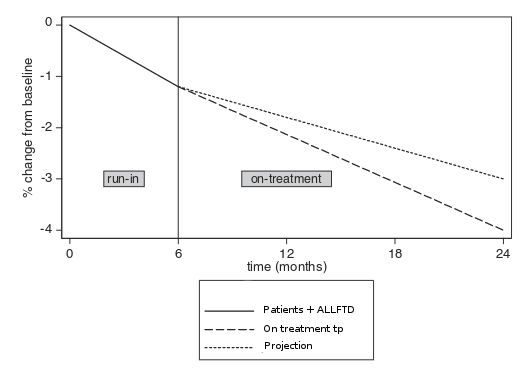
\includegraphics[scale=0.5, angle=0]{images/Run-in_run.png}
  \label{fig:Run_in}
\end{figure}

%%%%%%%%%%%%%%%%%%%%%%%%%%%%%%%%%%%%%%%%%%%%%%%%%%%%%%%%%%%%%%%%%%%%%%%%%%
\subsubsection{Sample size calculation for randomized controlled trials analysed using linear mixed models}

A general formulation for a linear mixed model is $Y|u \sim \mathcal{N}\left[ X\beta + Zu ; R\right]$ with $u \sim \mathcal{N}[0;G]$. This implies, marginally, that $Y \sim \mathcal{N}\left[ X\beta ; \Sigma\right]$ with $\Sigma = R + ZGZ^{T}$. Here $Y$ is the vector of outcome variables, $X$ is the design matrix, $\beta$ is the vector of fixed effects and $\Sigma$ is the variance-covariance matrix for the residuals. If a linear mixed model is to be used to analyse a randomized controlled trial then one of the elements of $\beta$ will correspond to a treatment effect. In order to carry out sample size calculations for such a trial it is necessary to specify both a postulated value for the estimated treatment effect and its anticipated standard error. Provided that there is a postulated fixed value for the variance-covariance matrix (which we will henceforth denote by $\Sigma$) then standard formulae for the contrasts yielding the parameter estimates (including the treatment effect) and the variance of these parameter estimates are given by $\hat{\beta} = (X^{T}\Sigma^{-1}X)^{-1}X^{T}\Sigma^{-1}Y$ and $V(\hat{\beta}) = (X^{T}\Sigma^{-1}X)^{-1}$.

%%%%%%%%%%%%%%%%%%%%%%%%%%%%%%%%%%%%%%%%%%%%%%%%%%%%%%%%%%%%%%%%%%%%%%%%%%
\subsubsection{Linear mixed models for randomized trials with a baseline measure of the outcome}

We consider a conventional two-group randomized controlled trial. Suppose $Y_{i0}$ an $Y_{i1}$ outcomes measured at follow-up and baseline for subject $i$ with randomization group indicated by $g_{i}$ , taking values 0 and 1.

\begin{equation*}
  \left(
  \begin{array}{c}
    Y_{i0} \\
    Y_{i1}
  \end{array}
  \right) \sim \mathcal{N} \left[ X\beta | \Sigma \right]= \mathcal{N} \left[
    \left(
    \begin{array}{ccc}
      1 & 0 & 0 \\
      0 & 1 & g_{i}
    \end{array}
    \right)
    \left(
    \begin{array}{c}
      \alpha_{0} \\
      \alpha_{1} \\
      \gamma
    \end{array}
    \right) |
    \left(
    \begin{array}{cc}
      \sigma_{1}^{2} & \sigma_{12} \\
      \sigma_{12}   & \sigma_{2}^{2}
    \end{array}
    \right)
  \right]
\end{equation*}

Provided that $\sigma_{1,2}^{2} > \sigma_{12}$, that implies that $\sigma_{1} = \sigma_{2}$. Then equation the model can be re-expressed as a linear mixed model as follows:

\begin{strip}
\begin{equation*}
  \left(
  \begin{array}{c}
    Y_{i0} \\
    Y_{i1}
  \end{array}
  \right) \sim \mathcal{N} \left[ X\beta + Zu| R \right]= \mathcal{N} \left[
    \left(
    \begin{array}{ccc}
      1 & 0 & 0 \\
      0 & 1 & g_{i}
    \end{array}
    \right)
    \left(
    \begin{array}{c}
      \alpha_{0} \\
      \alpha_{1} \\
      \gamma
    \end{array}
    \right) + \left(
    \begin{array}{cc}
      1 & 0 \\
      0 & 1
    \end{array}
    \right)\left(
    \begin{array}{c}
      u_{i}  \\
      u_{i} 
    \end{array}
    \right)|
    \left(
    \begin{array}{cc}
      \sigma_{1}^{2}-\sigma_{12} & 0 \\
      0                        & \sigma_{2}^{2}-\sigma_{12}
    \end{array}
    \right)
  \right]
\end{equation*}
\end{strip}

We can verify that $\Sigma = R + ZGZ^{T}$. The random effects $u_{i} \sim \mathcal{N}[0; G = \sigma_{12}]$ allow for the correlation between observations on the same subject in the two periods while the inclusion of the interaction between treatment and period, without a main effect of treatment, ensures that the treatment is only allowed to influence outcome at follow-up.

\subsubsection{Allowing for dropouts}

\subsubsection{Example 1: designs with three evenly spaced time points analysed with a standard random slopes model and assuming no dropouts}

To illustrate the methodology, first consider designs where measurements of outcome are made at baseline and at two evenly spaced subsequent visits. In our initial exposition, we use only the two changes between consecutive visits to estimate treatment effects. We do this because the exposition and resultant formulae are readily interpretable and because in many settings the additional gain in precision obtained by adjusting for baseline is small. Next Section, we show how baseline measures can be incorporated, and the impact that this has on the results.

\paragraph{Conventional designs}{First, consider a conventional design in which subjects ($i$) are randomized to two groups ($g_{i}$ = 0,1) of equal size and a continuous outcome is measured at baseline ($Y_{i0}$ at time $t_{0} = 0$) and two evenly spaced follow-up times ($Y_{i1}$, $Y_{i2}$ at $t_{1} = t$ and $t_{2} = 2t$, respectively). Assuming that the effect of treatment is to modify the rate of change a simple model for the data is

\begin{equation*}
  Y_{ij}|a_{i}, b_{i} \sim \mathcal{N} \left[
    \left(
    \begin{array}{ccc}
      1 & t_{j} & t_{j}g_{i}
    \end{array}
    \right)
    \left(
    \begin{array}{c}
      \alpha \\
      \beta \\
      \gamma
    \end{array}
    \right) +     \left(
    \begin{array}{cc}
      1 & t_{j}
    \end{array}
    \right)
    \left(
    \begin{array}{c}
      a_{i} \\
      b_{i}
    \end{array}
    \right) ; \sigma^{2}
    \right]
\end{equation*}

with the random effects define with:

\begin{equation*}
  \left(
  \begin{array}{c}
    a_{i} \\
    b_{i}
  \end{array}
  \right) \sim \mathcal{N} \left[
      \left(
  \begin{array}{c}
    0 \\
    0
  \end{array}
  \right) ;  \left(
  \begin{array}{cc}
    \sigma_{a}^{2} & \sigma_{ab} \\
    \sigma_{ab} & \sigma_{b}^{2}
  \end{array}
  \right) 
    \right]
\end{equation*}

Consideration of only the changes between successive visits, $C_{ij} = Y_{ij} - Y_{i(j-1)}$ reduces the number of parameters that need to be specified in a sample size calculation as

\begin{equation*}
  \left(
  \begin{array}{c}
    C_{i1} \\
    C_{i2}
  \end{array}
  \right) \sim \mathcal{N} \left[
      \left(
  \begin{array}{cc}
    t & tg_{i} \\
    t & tg_{i}
  \end{array}
  \right)\left(
  \begin{array}{c}
    \beta \\
    \gamma
  \end{array}
  \right) + \left(
  \begin{array}{c}
    t  \\
    t 
  \end{array}
  \right)\left(
  \begin{array}{c}
    b_i
  \end{array}
  \right) ;  \left(
  \begin{array}{cc}
    2\sigma^{2} & -\sigma^{2} \\
    -\sigma^{2} & 2\sigma^{2}
  \end{array}
  \right) 
    \right]
\end{equation*}

To get the covariance matrix we use the formula for a sequence $X_{1}, \ldots, X_{n}$ of random variables in real-valued, and constants $a_{1},\ldots ,a_{n}$, we have

\begin{equation*}
  \sigma ^{2}\left( \sum _{i=1}^{n}a_{i}X_{i} \right) = \sum _{i=1}^{n}a_{i}^{2}\sigma ^{2}(X_{i})+2\sum _{i,j\,:\,i<j}a_{i}a_{j}\operatorname {cov} (X_{i},X_{j})
\end{equation*}

In our situation we have $a_{1} = 1$ and $a_{2} = -1$. Solving $\hat{\beta} = (X^{T}\Sigma^{-1}X)^{-1}X^{T}\Sigma^{-1}Y$ and $V(\hat{\beta}) = (X^{T}\Sigma^{-1}X)^{-1}$ for this model as used to analyse data from a hypothetical two-person trial where $g_{1} = 0$ and $g_{2} = 1$ gives $\hat{\gamma} = [(C_{22} + C_{21}) -(C_{12} + C_{11})]/(2t)$ and $V(\hat{\gamma}) = 2\sigma_{b}^{2} + \sigma^{2}/t^{2}$. Here, as is intuitive, the treatment effect is just the difference in the sum of the two changes between the two subjects. As the follow-up time increases, the variance of the treatment difference declines to an asymptote defined by the between-subject variance in atrophy rates.}

\paragraph{Run-in designs}{Now suppose that subjects are only randomized at the second of the three visits. Assuming the same within-subject covariance structure, as the previouse paragraph, a model for the consecutive changes that forces a common slope ($\delta$) in the pre-randomization periods, but allows different slopes in the post-randomization periods ($\beta$ and $\beta+\gamma$, respectively) is

  \begin{equation*}
    \left(
    \begin{array}{c}
      C_{i1} \\
      C_{i2}
    \end{array}
    \right) \sim \mathcal{N}\left[ \left(
      \begin{array}{ccc}
        t & 0 & 0 \\
        0 & t & tg_{i}
      \end{array}
      \right) \left(
      \begin{array}{c}
        \delta \\
        \beta \\
        \gamma
      \end{array}
      \right) + \left(
      \begin{array}{c}
        t \\
        t
      \end{array}
      \right) \left(
      \begin{array}{c}
        b_{i}
      \end{array}
      \right) ; \left(
  \begin{array}{cc}
    2\sigma^{2} & -\sigma^{2} \\
    -\sigma^{2} & 2\sigma^{2}
  \end{array}
  \right) \right]
  \end{equation*}

  In practice, in order to perform an analysis that yields identical results to an analysis of covariance, it might be advisable to allow the variance of the changes in the two periods to differ. However, for the purposes of carrying out sample size calculations, and in the absence of data, it is reasonable to assume that these variances are the same. Solving $\hat{\beta} = (X^{T}\Sigma^{-1}X)^{-1}X^{T}\Sigma^{-1}Y$ and $V(\hat{\beta}) = (X^{T}\Sigma^{-1}X)^{-1}$ this model gives the following formulae for the estimated treatment effect and its variance: $\hat{\gamma} = ((C_{22} - C_{12})-r(C_{21} - C_{11}))/t$ and

  $$
  V(\hat{\gamma}) = \left( \frac{\sigma^{2}}{t^{2}} + 2\sigma_{b}^{2} \right)(1-r),~~where~r = \frac{t^{2}\sigma_{b}^{2} - 2\sigma^{2}}{t^{2}\sigma_{b}^{2} + 2\sigma^{2}} 
  $$

Here the treatment effect is the difference in rates in the second period corrected for any difference in baseline rates where the extent of the correction is determined by the correlation between the rates in the two periods ($r$). In contrast to a conventional design the efficiency of the run-in design is not bounded by an asymptote as the time interval between visits increases.
}

%%%%%%%%%%%%%%%%%%%%%%%%%%%%%%%%%%%%%%%%%%%%%%%%%%%%%%%%%%%%%%%%%%%%%%%%%%
%%%%%%%%%%%%%%%%%%%%%%%%%%%%%%%%%%%%%%%%%%%%%%%%%%%%%%%%%%%%%%%%%%%%%%%%%%
\section{discussion}

%%%%%%%%%%%%%%%%%%%%%%%%%%%%%%%%%%%%%%%%%%%%%%%%%%%%%%%%%%%%%%%%%%%%%%%%%%
\subsection{Article}

\begin{enumerate}
  \item {\it Bayesian Mixted Linear Effect for longitudinal structural study of neuroimaging in FTD}. Study of variance reduction. What sort of prior information in the first time-point could bring the variance down. Priors could be chosen like CDR, DTI region of interests in the white matter, ASL, \dots
  \item {\it Bayesian Mixted Linear Effect for longitudinal ASL study on gene carriers}. Study of the C9, GRN and map-t for symptomatic and asymptomatic patients "Luke as a first author".
  \item {\it Bayesian Mixted Linear Effect for longitudinal ASL and PET study}. Study of the the overlapping set of data between PET and ASL.
  \item {\it Model based rate of atrophy on LEFFTDs data}. Bayesian Mixted Linear Effect on the longitudinal LEFFTDs/NITFD data.
\end{enumerate}


%%%%%%%%%%%%%%%%%%%%%%%%%%%%%%%%%%%%%%%%%%%%%%%%%%%%%%%%%%%%%%%%%%%%%%%%%%
%%%%%%%%%%%%%%%%%%%%%%%%%%%%%%%%%%%%%%%%%%%%%%%%%%%%%%%%%%%%%%%%%%%%%%%%%%
\section{Conclusion}

\section*{References}
%% References with bibTeX database:
\bibliographystyle{Bibliography/elsarticle-num}

\bibliography{Bibliography/sample}


\end{document}
